% !TEX root = ../../../main.tex
% 来源：中学数学实验教材·第三册（高中数学）
% 章节：函数及其图象 / 一次函数（线性函数）
% 原始文件：4.tex，行 1726-1733
% 类型：tikz
% ---
    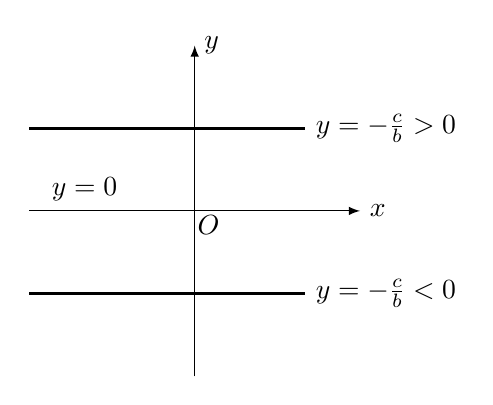
\begin{tikzpicture}[>=latex, scale=.7]
        \draw[->](-3,0)--(3,0)node[right]{$x$};
        \draw[->] (0,-3)--(0,3)node[right]{$y$};
    \draw[very thick] (-3,1.5)--(2,1.5)node[right]{$y=-\frac{c}{b}>0$};
    \draw[very thick] (-3,-1.5)--(2,-1.5)node[right]{$y=-\frac{c}{b}<0$};
    \node at (-2,0)[above]{$y=0$};
    \node at (.25,-.25){$O$};
    \end{tikzpicture}
